\chapter{Fundamentação Teórica}
\label{cap:fund}

Este capítulo reúne os conceitos usados no restante do trabalho. Começa pelas imagens hiperespectrais e pela redução de dimensionalidade, passa pelo processamento de imagens, pela segmentação por superpixels e pelas métricas de avaliação, e chega ao aprendizado de máquina e às redes neurais convolucionais unidimensionais usadas na classificação espectral. Em seguida trata do processamento paralelo em GPUs, da concorrência em CPU e da otimização de hiperparâmetros, e termina com os trabalhos relacionados que servem de ponto de partida para a proposta.

\section{Imagem Hiperespectral}

A imagem hiperespectral (HSI), dado de entrada da classificação estudada neste trabalho, combina espectroscopia e imagem e registra informação tanto no domínio espacial quanto no espectral \cite{Li2019DeepLF}. Imagens multiespectrais capturam poucas bandas largas do espectro; as HSIs registram centenas de bandas estreitas e contíguas, tipicamente na faixa de 400 a 2500 nanômetros \cite{Qian2020}, o que permite analisar em detalhe a composição dos materiais de uma cena. O espectro eletromagnético pode ser organizado pela energia por fóton, dos raios gama (maior energia) às ondas de rádio (menor energia) \cite{gonzalez2018digital}. A Figura \ref{fig:landsat_bands} mostra imagens multiespectrais do satélite LANDSAT da área de Washington D.C., uma por banda temática. Cada banda serve a um uso: a do azul visível é a que mais penetra na água, e a do infravermelho próximo é usada no mapeamento de biomassa e de linhas de costa \cite{gonzalez2018digital}. A HSI leva essa separação a centenas de bandas e tem aplicações em sensoriamento remoto, agricultura de precisão e diagnóstico médico \cite{Lurs12162659}.

\begin{figure}[H]
    \centering
    \captionsetup{justification=centering}
    \caption{Imagens de satélite LANDSAT da área de Washington D.C. em diferentes bandas espectrais temáticas}
    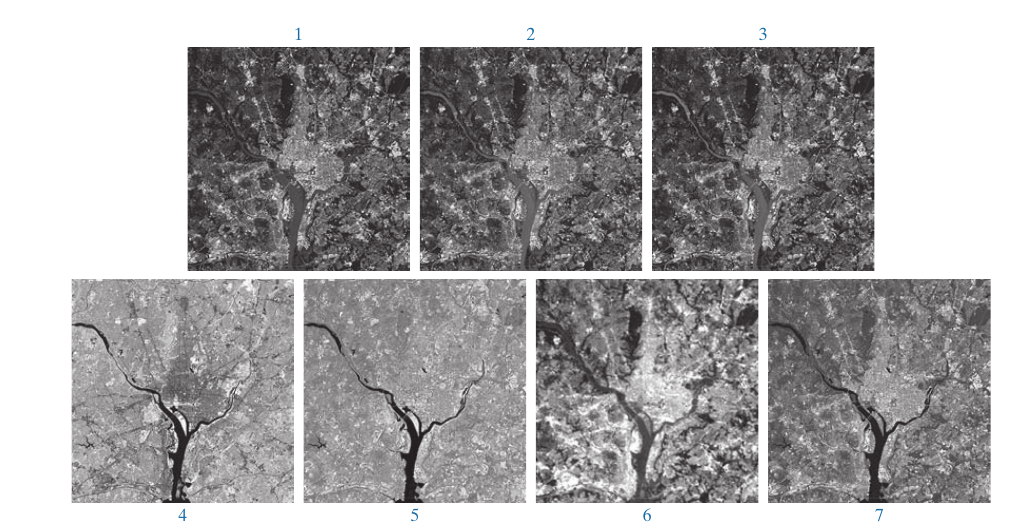
\includegraphics[width=0.8\textwidth]{src/assets/fundamentacao/landsat_bands.png}
    \captionsetup{justification=raggedright}
    \caption*{Fonte: \citefigure{gonzalez2018digital}}
    \label{fig:landsat_bands}
\end{figure}

Uma HSI tem alta resolução espectral, mas baixa resolução espacial \cite{Viel2019}, porque o sensor concentra a captura de cada ponto da cena em centenas de bandas estreitas e contíguas. A Figura \ref{fig:hsi_structure} mostra como o dado se forma: a plataforma do sensor, em movimento, captura linhas de varredura sucessivas, que são empilhadas em um hipercubo com duas dimensões espaciais e uma espectral.

\begin{figure}[H]
    \centering
    \captionsetup{justification=centering}
    \caption{Estrutura de dados de uma imagem hiperespectral: (a) aquisição por sensor em movimento; (b) formação do hipercubo tridimensional; (c) dimensões espaciais e canais espectrais}
    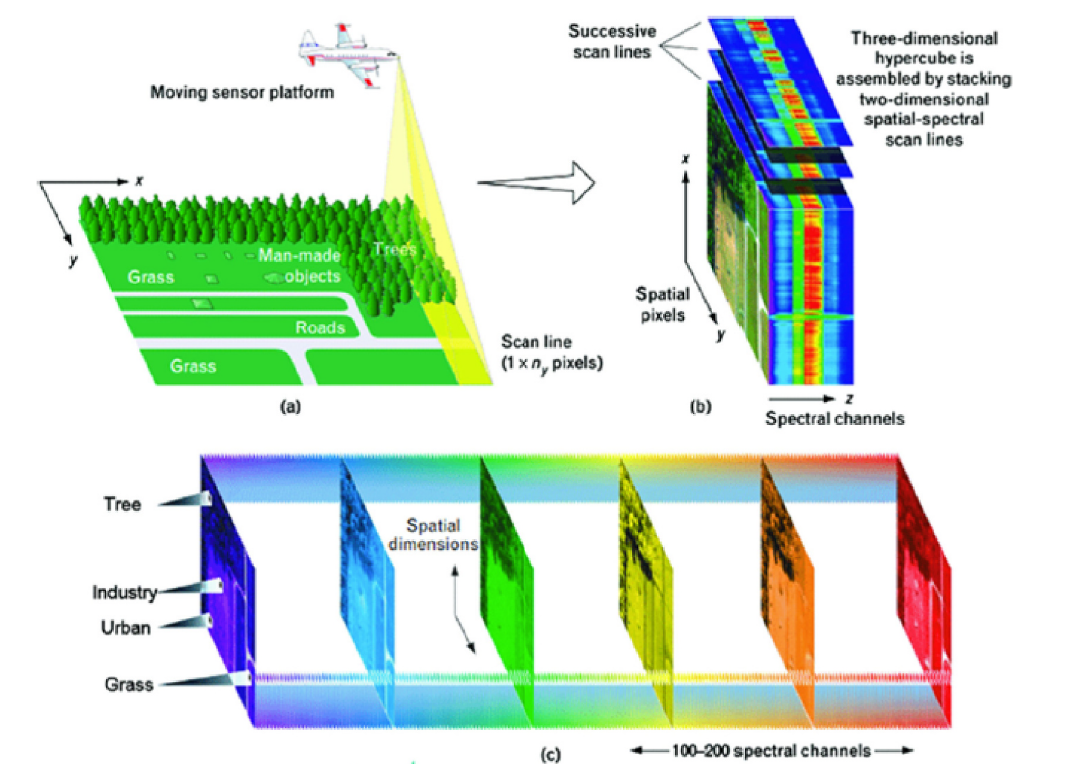
\includegraphics[width=0.75\textwidth]{src/assets/fundamentacao/hsi_structure.png}
    \captionsetup{justification=raggedright}
    \caption*{Fonte: \citefigure{Qian2020}}
    \label{fig:hsi_structure}
\end{figure}

A alta dimensionalidade das HSIs traz três desafios principais à sua análise: (1) a alta redundância de dados, causada pela forte correlação entre bandas espectrais adjacentes; (2) a variabilidade das assinaturas hiperespectrais, que podem mudar com as condições atmosféricas ou de iluminação; e (3) a maldição da dimensionalidade (\textit{curse of dimensionality}), em que o grande número de bandas prejudica o desempenho dos algoritmos de classificação e exige um número exponencialmente maior de amostras de treinamento \cite{Ahmad_2025}. As etapas básicas da análise de HSIs incluem pré-processamento, extração e seleção de características, e classificação ou desmistura (\textit{unmixing}) espectral.

\subsection{Redução de Dimensionalidade}

O número de bandas das HSIs e a correlação entre bandas adjacentes motivam a redução de dimensionalidade antes da classificação. A Análise de Componentes Principais (PCA) projeta os dados sobre as direções de maior variância e, com poucas componentes, preserva a maior parte da variância dos dados originais \cite{Jolliffe2002}. A projeção é definida pela equação:

\begin{equation}
z_i^t = w_i^T x^t, \quad i=1,\ldots,k, \quad t=1,\ldots,N
\end{equation}
\addEquacao{Projeção PCA}{6}

\noindent onde $x^t$ são os dados de entrada do pixel $t$, $w_i$ são os autovetores correspondentes aos maiores autovalores, $z_i^t$ são as componentes principais projetadas, $k$ é o número de componentes principais retidas, e $N$ é o número total de pixels. O algoritmo envolve: (1) centralização dos dados, subtraindo a média espectral; (2) cálculo da matriz de covariância; (3) decomposição da matriz de covariância em autovetores e autovalores; e (4) projeção dos dados originais nos autovetores correspondentes aos maiores autovalores \cite{Jolliffe2002}. Neste trabalho, o número $k$ de componentes retidas é um dos hiperparâmetros do espaço de busca (\autoref{qua:espaco}).

\section{Processamento de Imagens}

Uma imagem pode ser definida como uma função bidimensional, $f(x, y)$, onde $x$ e $y$ são coordenadas espaciais, e a amplitude de $f$ em qualquer par de coordenadas $(x, y)$ é chamada de intensidade ou nível de cinza da imagem naquele ponto \cite{gonzalez2018digital}. Quando $x$, $y$ e os valores de intensidade de $f$ são quantidades finitas e discretas, a imagem é chamada de imagem digital. O campo do processamento digital de imagens refere-se ao processamento de imagens digitais por meio de um computador digital.

O processamento de imagens pode ser categorizado em três níveis: baixo nível (pré-processamento, redução de ruído, realce de contraste), nível médio (segmentação, descrição de objetos, classificação) e alto nível (análise de cena e reconhecimento) \cite{gonzalez2018digital}. A Figura \ref{fig:erosion_example} exemplifica uma operação morfológica de erosão, um tipo de processamento de baixo nível comumente utilizado para remover componentes indesejados de imagens binárias.

\begin{figure}[H]
    \centering
    \captionsetup{justification=centering}
    \caption{Exemplo de operação de erosão morfológica aplicada a uma imagem binária usando elementos estruturantes de diferentes tamanhos}
    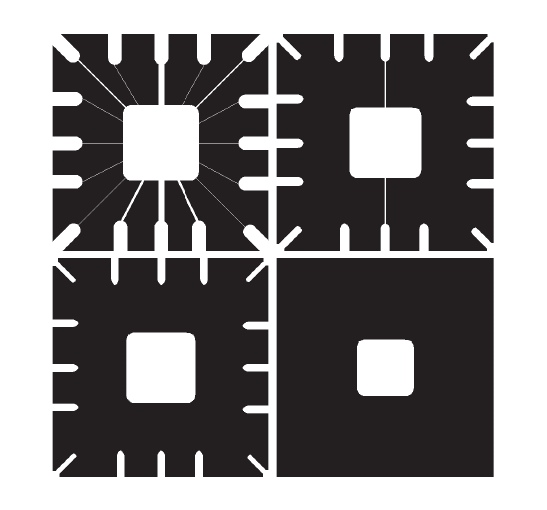
\includegraphics[width=0.55\textwidth]{src/assets/fundamentacao/erosion_example.png}
    \captionsetup{justification=raggedright}
    \caption*{Fonte: \citefigure{gonzalez2018digital}}
    \label{fig:erosion_example}
\end{figure}

A Figura \ref{fig:segmentation_cells} exemplifica o processamento de nível médio, mostrando a segmentação e identificação de células individuais em imagens microscópicas.

\begin{figure}[H]
    \centering
    \captionsetup{justification=centering}
    \caption{Exemplo de processamento de nível médio: segmentação de células em imagens microscópicas}
    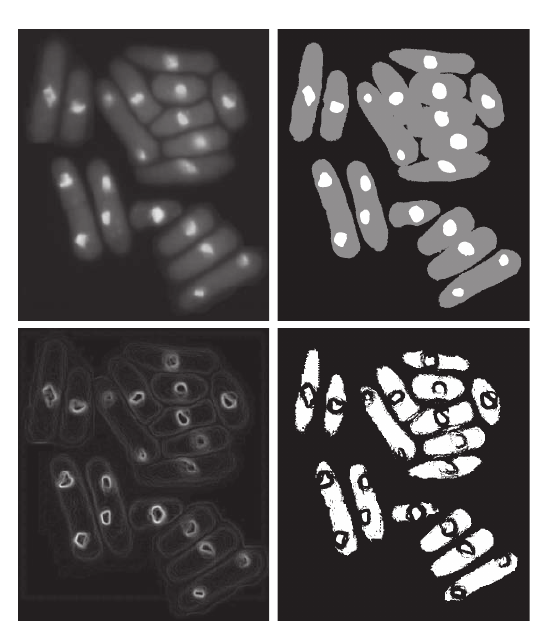
\includegraphics[width=0.5\textwidth]{src/assets/fundamentacao/segmentation_cells.png}
    \captionsetup{justification=raggedright}
    \caption*{Fonte: \citefigure{gonzalez2018digital}}
    \label{fig:segmentation_cells}
\end{figure}

A Figura \ref{fig:sift_matching} exemplifica o processamento de alto nível, mostrando o reconhecimento e correspondência de características entre imagens usando o algoritmo SIFT.

\begin{figure}[H]
    \centering
    \captionsetup{justification=centering}
    \caption{Exemplo de processamento de alto nível: correspondência de características usando SIFT, mostrando 41 pares encontrados com apenas 3 erros reais}
    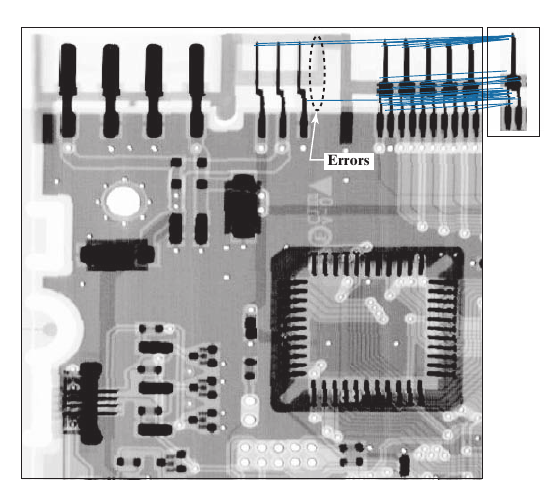
\includegraphics[width=0.55\textwidth]{src/assets/fundamentacao/sift_matching.png}
    \captionsetup{justification=raggedright}
    \caption*{Fonte: \citefigure{gonzalez2018digital}}
    \label{fig:sift_matching}
\end{figure}

\subsection{Segmentação de Imagens}
\label{subsec:fundSegmentacao}

No fluxo de classificação deste trabalho, a segmentação extrai a informação espacial que complementa as características espectrais. A segmentação de imagens é o processo de particionar uma imagem em múltiplos segmentos ou regiões de interesse \cite{FENG2019309}, e sua função é simplificar a representação da imagem em algo mais fácil de analisar. No domínio das HSIs, a segmentação usa a informação espacial para auxiliar a classificação, o que é útil quando objetos distintos apresentam assinaturas espectrais parecidas, mas estruturas geométricas ou texturas diferentes \cite{Souza2023}. Em Indian Pines, por exemplo, milho e soja aparecem cada um em três classes, conforme o manejo do solo; os espectros dessas classes diferem pouco entre si, mas cada uma ocupa talhões contíguos, e a região a que o pixel pertence pode ajudar a separar o que o espectro sozinho confunde. A Figura \ref{fig:segmentation_types} ilustra os dois principais tipos de mapa de segmentação gerados pelo algoritmo SEEDS: o mapa de bordas, que identifica os contornos entre superpixels, e o mapa de regiões, que atribui rótulos únicos a cada segmento homogêneo da imagem.

\begin{figure}[H]
    \centering
    \captionsetup{justification=centering}
    \caption{Tipos de mapa de segmentação: bordas (superior) e regiões (inferior) gerados pelo algoritmo SEEDS}
    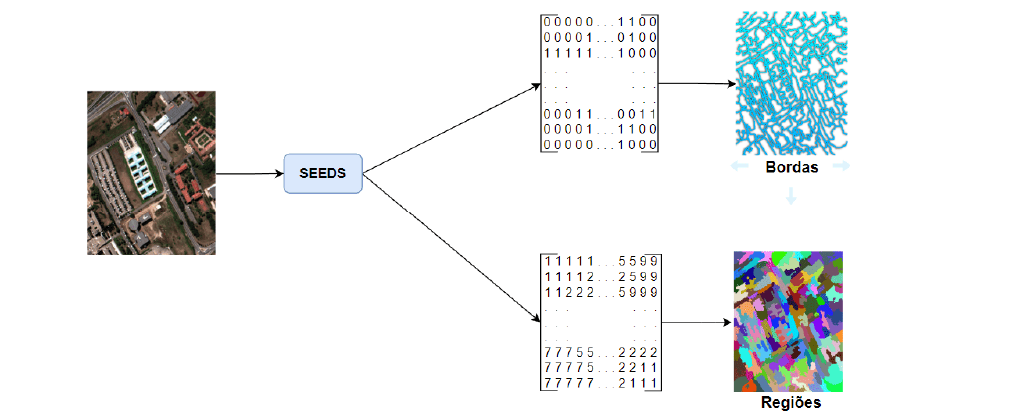
\includegraphics[width=0.85\textwidth]{src/assets/fundamentacao/segmentation_types.png}
    \captionsetup{justification=raggedright}
    \caption*{Fonte: \citefigure{Souza2023}}
    \label{fig:segmentation_types}
\end{figure}

Um método de segmentação morfológica utiliza os resíduos de transformadas de abertura e fechamento morfológicas baseadas em uma métrica geodésica \cite{Pesaresi905239}. Essa abordagem introduz o conceito de nivelamento (\textit{leveling}). A reconstrução em tons de cinza de uma imagem $g$ a partir de um marcador $f$ é obtida pelo uso iterativo de dilatações geodésicas elementares até a idempotência:

\begin{equation}
R_g^\delta(f) = \delta_g^{(i)}(f)
\end{equation}
\addEquacao{Reconstrução Geodésica Morfológica}{7}

\noindent onde $R_g^\delta(f)$ é a reconstrução geodésica do marcador $f$ sob a imagem de referência $g$, e $\delta_g^{(i)}(f)$ representa a dilatação geodésica elementar aplicada iterativamente até atingir idempotência (estabilidade). A característica morfológica multiescala de um ponto na imagem é definida pelo tamanho do elemento estruturante que possui o maior valor associado na derivada do perfil morfológico. O vetor da derivada do perfil morfológico (DMP) é:

\begin{equation}
\Delta(x) = (\Delta_0(x), ..., \Delta_\lambda(x), ..., \Delta_N(x))
\end{equation}
\addEquacao{Vetor de Derivada do Perfil Morfológico (DMP)}{8}

\noindent onde $\Delta(x)$ é o vetor de derivadas do perfil morfológico no ponto $x$, $\Delta_\lambda(x)$ representa a derivada para o elemento estruturante de tamanho $\lambda$, e $N$ é o número total de escalas.

O SEEDS (\textit{Superpixels Extracted via Energy-Driven Sampling}) parte de uma partição da imagem em grade regular e refina as fronteiras dos superpixels por \textit{hill-climbing}: blocos de pixels, e depois pixels isolados, passam para um superpixel vizinho sempre que a troca aumenta uma função de energia \cite{bergh2013seedssuperpixelsextractedenergydriven}:

\begin{equation}
E(s) = H(s) + \gamma G(s)
\end{equation}
\addEquacao{Função de Energia do Algoritmo SEEDS}{9}

\noindent onde $E(s)$ é a energia da segmentação $s$, $H(s)$ é o termo de histograma, que mede a homogeneidade de cor dentro de cada superpixel, $G(s)$ é o termo de contorno, que favorece fronteiras suaves, e $\gamma$ controla o equilíbrio entre cor e contornos.

Além do SEEDS, três outros algoritmos de superpixels são usados neste trabalho. O SLIC (\textit{Simple Linear Iterative Clustering}) distribui sementes em uma grade regular de espaçamento $S$ e executa um \textit{k-means} local, em que cada pixel é atribuído à semente mais próxima segundo uma distância que combina cor e posição; a busca de cada semente fica restrita a uma janela de $2S \times 2S$ ao seu redor \cite{Achanta2012SLIC}. A variante SLICO ajusta a compacidade automaticamente, dispensando o parâmetro que a controla. O LSC (\textit{Linear Spectral Clustering}) mapeia cada pixel para um espaço de características de dimensão mais alta, no qual um \textit{k-means} ponderado aproxima o critério de cortes normalizados em grafos, o que tende a produzir bordas mais aderentes aos contornos da imagem \cite{Zhengqin7298741}. O Watershed trata a magnitude do gradiente como um relevo topográfico e o inunda a partir de marcadores; as fronteiras entre regiões surgem onde águas de bacias diferentes se encontram \cite{Najman546254}. Todos eles, assim como o SEEDS, recebem como entrada uma imagem de três canais: no caso das HSIs, uma composição das três primeiras componentes principais.

\subsection{Métricas de Avaliação}

As métricas de classificação de HSIs derivam da matriz de confusão, que cruza, para cada pixel avaliado, a classe verdadeira com a classe prevista \cite{Congalton1991}. Sejam $n_{ij}$ o número de pixels da classe verdadeira $i$ atribuídos à classe $j$, $c$ o número de classes, $N$ o total de pixels avaliados, e $n_{i+} = \sum_{j} n_{ij}$ e $n_{+i} = \sum_{j} n_{ji}$ os totais da linha e da coluna da classe $i$. As três métricas usadas neste trabalho são as seguintes.

\textbf{Acurácia Geral (Overall Accuracy - OA):}

\begin{equation}
OA = \frac{1}{N} \sum_{i=1}^{c} n_{ii}
\end{equation}
\addEquacao{Acurácia Geral (OA)}{10}

\noindent isto é, a proporção de pixels classificados corretamente \cite{Congalton1991}. Com duas classes, a expressão se reduz a $(vp + vn)/(vp + vn + fp + fn)$, em que $vp$, $vn$, $fp$ e $fn$ são os verdadeiros positivos, os verdadeiros negativos, os falsos positivos e os falsos negativos.

\textbf{Acurácia Média (Average Accuracy - AA):}

\begin{equation}
AA = \frac{1}{c} \sum_{i=1}^{c} \frac{n_{ii}}{n_{i+}}
\end{equation}
\addEquacao{Acurácia Média (AA)}{11}

\noindent onde $n_{ii}/n_{i+}$ é a acurácia da classe $i$, isto é, a fração dos seus pixels classificada corretamente. Como cada classe pesa o mesmo, a AA pune o classificador que acerta só as classes grandes. Por exemplo, um classificador que acerta 85 dos 90 pixels de uma classe frequente, mas só 4 dos 10 pixels de uma classe rara e 8 dos 10 de outra, tem OA de 0,88 e AA de 0,71. Em Indian Pines, cujas classes vão de 20 a 2.455 pixels rotulados, a distância entre as duas métricas é grande.

\textbf{Coeficiente Kappa ($\kappa$):}

\begin{equation}
\kappa = \frac{p_o - p_e}{1 - p_e}
\end{equation}
\addEquacao{Coeficiente Kappa}{12}

\noindent onde $p_o$ é a concordância observada, igual à OA, e $p_e = \frac{1}{N^2} \sum_{i=1}^{c} n_{i+}\, n_{+i}$ é a concordância esperada por acaso, calculada pelos totais de linha e de coluna. Proposto por \citeonline{Cohen1960}, o coeficiente mede a concordância entre a classificação e o Ground Truth (GT) descontando a parcela que ocorreria por acaso: vale 1 para concordância perfeita e 0 quando a concordância é a esperada por acaso \cite{Congalton1991}.

\section{Aprendizado de Máquina}

O Aprendizado de Máquina, do inglês \textit{Machine Learning} (ML), é o campo de estudo que dá aos computadores a capacidade de aprender sem serem explicitamente programados \cite{SomeStudiesinMachineLearningUsingtheGameofCheckers}. O aprendizado profundo, ao qual pertencem as CNNs usadas neste trabalho, é um de seus ramos \cite{DeeplearningLC}. Um programa de computador aprende a partir de uma experiência ($E$) com respeito a uma classe de tarefas ($T$) e uma medida de desempenho ($P$) se o seu desempenho nas tarefas em $T$, medido por $P$, melhora com a experiência $E$ \cite{MachineLearning}. A Figura \ref{fig:checkers_tree} mostra um exemplo clássico, o programa de damas de \citeonline{SomeStudiesinMachineLearningUsingtheGameofCheckers}, que avalia os movimentos possíveis por meio de uma árvore de jogadas e escolhe o ramo de maior pontuação.

\begin{figure}[H]
    \centering
    \captionsetup{justification=centering}
    \caption{Diagrama simplificado mostrando como as avaliações são respaldadas através da árvore de movimentos possíveis para chegar ao melhor próximo movimento}
    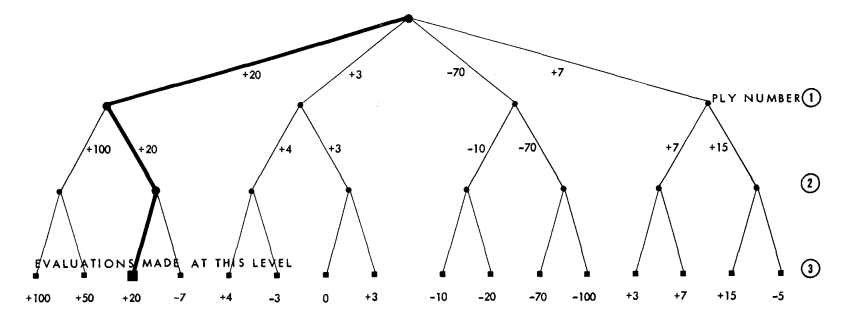
\includegraphics[width=0.75\textwidth]{src/assets/fundamentacao/checkers_tree.png}
    \captionsetup{justification=raggedright}
    \caption*{Fonte: \citefigure{SomeStudiesinMachineLearningUsingtheGameofCheckers}}
    \label{fig:checkers_tree}
\end{figure}

\subsection{Desafios Centrais: Generalização e Sobreajuste}

O desafio principal é garantir que o desempenho de um modelo ($P$) melhore não apenas nos dados de treinamento ($E$), mas também em dados novos. Quando isso não ocorre, há sobreajuste, do inglês \textit{overfitting} (OF): o modelo se ajusta demais aos dados de treinamento e captura ruído em vez do padrão subjacente \cite{Overfittingproblem:anewperspectivefromthegeometricalinterpretationofMLP}, com bom desempenho no treinamento e desempenho ruim em entradas novas. Por isso o desempenho é acompanhado em um conjunto de validação, separado do treino. A Figura \ref{fig:gradient_descent} traz um exemplo de \citeonline{DeepLearningIG}: durante o treino de uma rede convolucional, a norma do gradiente cresce, sinal de que o otimizador não chega a um ponto crítico, e ainda assim o erro de classificação na validação cai a um nível baixo. O que indica se o modelo generaliza é esse erro, medido fora do treino, e não a convergência do otimizador.

As estratégias de regularização restringem a complexidade efetiva do modelo para reduzir o OF \cite{DeepLearningIG}. Três delas aparecem neste trabalho: o \textit{dropout}, que desativa ao acaso uma fração dos neurônios a cada passo de treino e impede que eles se coadaptem \cite{Dropout:asimplewaytopreventneuralnetworksfromoverfitting}, usado nas duas camadas densas ocultas da rede; o \textit{weight decay}, que penaliza a norma dos pesos; e a parada antecipada, que interrompe o treino quando o desempenho na validação deixa de melhorar \cite{DeepLearningIG}.

\begin{figure}[H]
    \centering
    \captionsetup{justification=centering}
    \caption{Comportamento da descida de gradiente durante o treinamento de uma rede convolucional: (Esquerda) distribuição das normas do gradiente ao longo do tempo; (Direita) taxa de erro de classificação no conjunto de validação}
    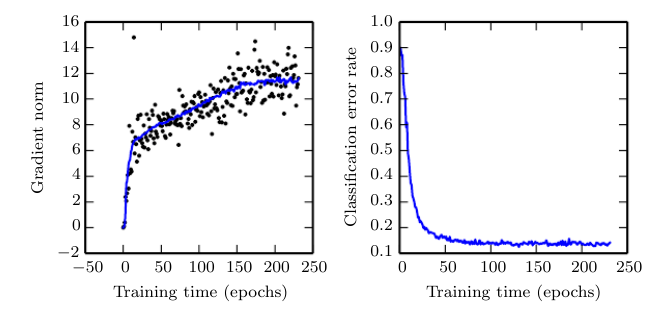
\includegraphics[width=0.85\textwidth]{src/assets/fundamentacao/gradient_descent_behavior.png}
    \captionsetup{justification=raggedright}
    \caption*{Fonte: \citefigure{DeepLearningIG}}
    \label{fig:gradient_descent}
\end{figure}

\subsection{Paradigmas de Aprendizagem}

A natureza dos dados e do problema determina qual paradigma de aprendizado usar \cite{WhatIsMachineLearning}. A Figura \ref{fig:learning_paradigms} ilustra os três principais paradigmas e a relação de cada um com o tipo de dado de treinamento.

\begin{figure}[H]
    \centering
    \captionsetup{justification=centering}
    \caption{Paradigmas de aprendizagem e sua relação com os tipos de dados de treinamento}
    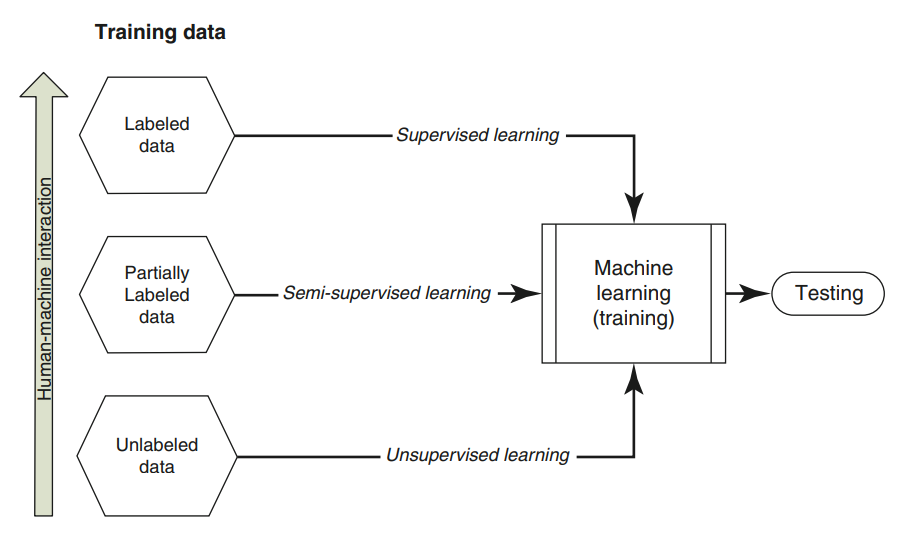
\includegraphics[width=0.65\textwidth]{src/assets/fundamentacao/learning_paradigms.png}
    \captionsetup{justification=raggedright}
    \caption*{Fonte: \citefigure{WhatIsMachineLearning}}
    \label{fig:learning_paradigms}
\end{figure}

\begin{itemize}
    \item \textbf{Aprendizado Supervisionado}: Estima um mapeamento a partir de amostras de entrada e saída, em que as saídas são rótulos ou valores conhecidos. As tarefas mais comuns são classificação e regressão. É o paradigma deste trabalho: cada pixel rotulado do GT fornece um espectro de entrada e a classe esperada.

    \item \textbf{Aprendizado Não Supervisionado}: O sistema recebe apenas amostras de entrada, sem rótulos, e procura estrutura nos próprios dados, como grupos de amostras semelhantes. Os algoritmos de superpixels SLIC e LSC (\autoref{subsec:fundSegmentacao}) são exemplos: agrupam pixels por \textit{k-means} sem usar nenhum rótulo.

    \item \textbf{Aprendizado Semissupervisionado}: Do inglês \textit{Semi-supervised learning} (SSL), situa-se entre os dois paradigmas anteriores e usa dados em que apenas parte das amostras é rotulada.
\end{itemize}

\subsection{Aprendizado Profundo}

Os sistemas tradicionais de reconhecimento de padrões eram formados por dois módulos: um extrator de características projetado manualmente e um classificador treinável, e o desempenho dependia da engenharia dessas características \cite{DeeplearningLC}. O Aprendizado Profundo, do inglês \textit{Deep Learning} (DL), remove essa dependência: modelos compostos por múltiplas camadas de processamento aprendem, diretamente dos dados brutos, representações com múltiplos níveis de abstração \cite{Asurveyonstate-of-the-artdeeplearningapplicationsandchallenges}. O DL é um método de aprendizado de representação obtido pela composição de módulos simples e não lineares, em que cada camada transforma a representação da camada anterior em uma de nível de abstração superior \cite{DeeplearningLC}. A Figura \ref{fig:cnn_architecture} ilustra a arquitetura de uma rede neural convolucional, com convoluções seguidas da função de ativação ReLU e camadas de \textit{max pooling} que reduzem progressivamente a dimensão espacial. As funções de ativação, como a Unidade Linear Retificada (ReLU), introduzem não linearidades na rede. A ReLU é definida como:

\begin{equation}
f(z) = \max(z, 0) = \begin{cases} 
z, & \text{se } z > 0 \\
0, & \text{caso contrário}
\end{cases}
\end{equation}
\addEquacao{Função de Ativação ReLU}{1}

\noindent onde $z$ é a entrada da função de ativação. Por não saturar para entradas positivas, a ReLU acelera o treino em relação a funções saturantes, como a sigmoide e a tangente hiperbólica: em uma rede convolucional de quatro camadas treinada no CIFAR-10, a versão com ReLU atingiu 25\% de erro de treino seis vezes mais rápido que a versão com tangente hiperbólica \cite{NIPS2012_c399862d}. O treinamento dessas redes usa o algoritmo de retropropagação, do inglês \textit{backpropagation}, que calcula o gradiente da função de perda em relação a cada peso da rede e permite ajustar os parâmetros por descida de gradiente \cite{Gradient-basedlearningappliedtodocumentrecognition}. A Figura \ref{fig:backpropagation} mostra como uma rede neural multicamadas pode distorcer o espaço de entrada para tornar as classes linearmente separáveis, e como a retropropagação aplica a regra da cadeia, tanto na propagação para frente (\textit{forward pass}) quanto na retropropagação dos gradientes (\textit{backward pass}).

\begin{figure}[H]
    \centering
    \captionsetup{justification=centering}
    \caption{Redes neurais multicamadas e backpropagation: (a) transformação do espaço de entrada; (b) regra da cadeia; (c) equações do forward pass; (d) equações do backward pass}
    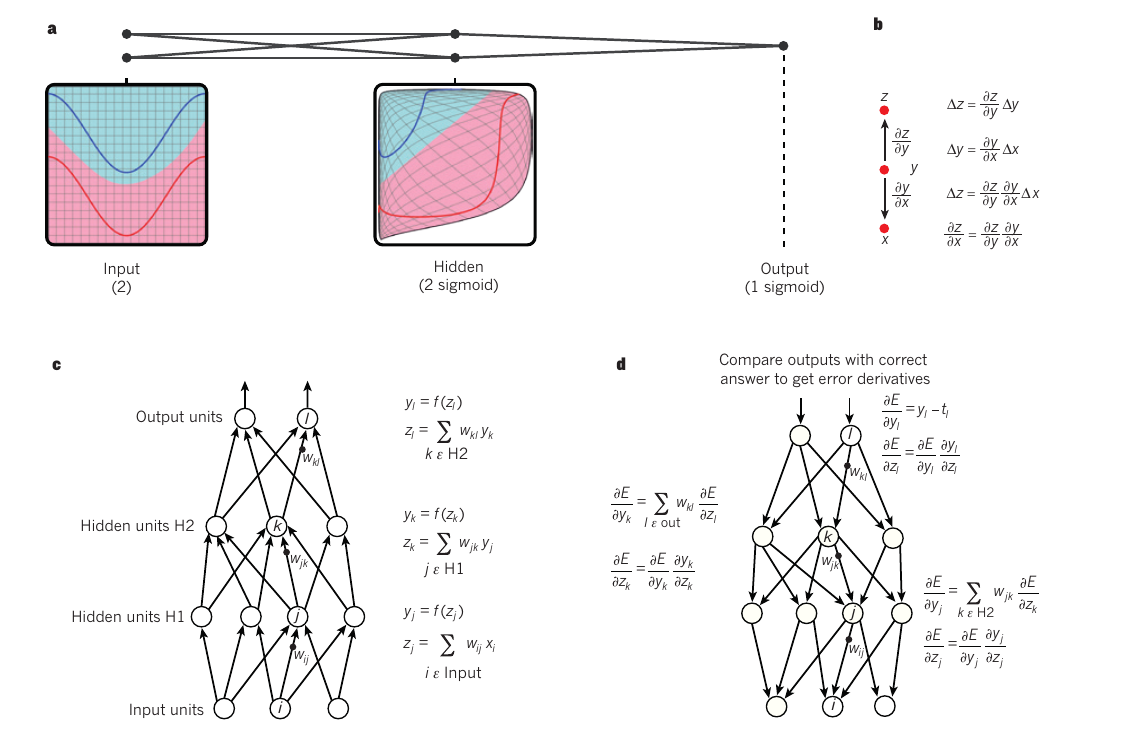
\includegraphics[width=0.75\textwidth]{src/assets/fundamentacao/backpropagation.png}
    \captionsetup{justification=raggedright}
    \caption*{Fonte: \citefigure{DeeplearningLC}}
    \label{fig:backpropagation}
\end{figure}

\begin{figure}[H]
    \centering
    \captionsetup{justification=centering}
    \caption{Arquitetura de uma rede neural convolucional mostrando camadas de convolução com ReLU e max pooling}
    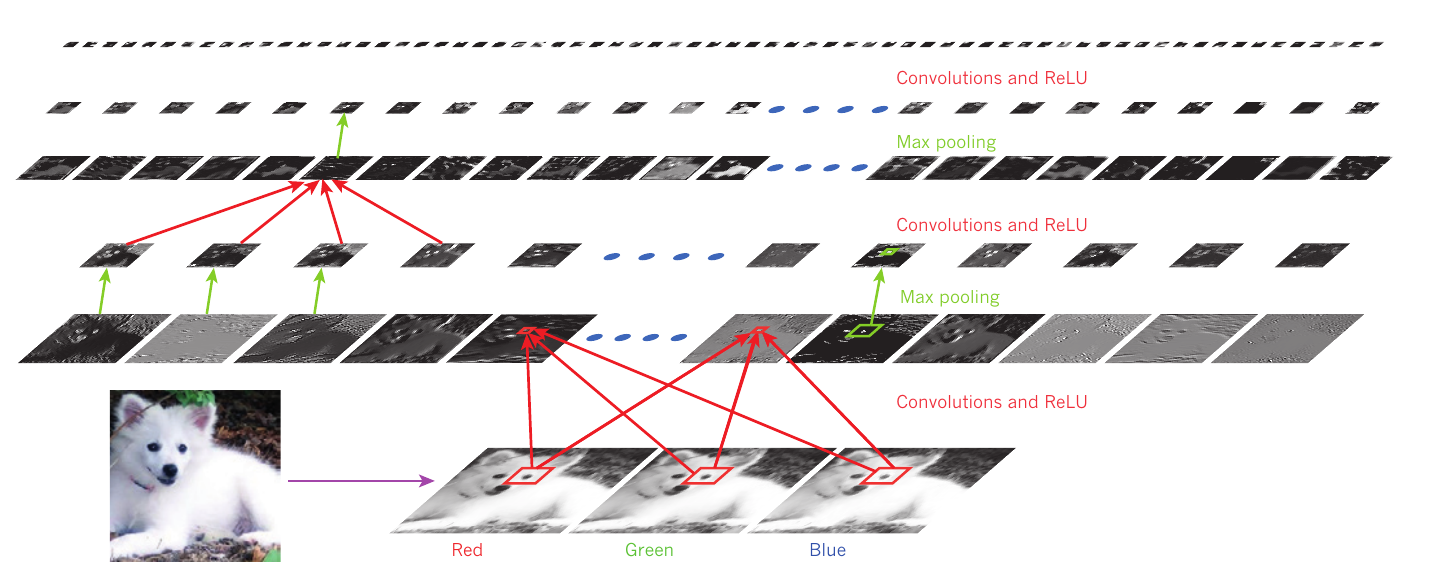
\includegraphics[width=0.9\textwidth]{src/assets/fundamentacao/cnn_architecture.png}
    \captionsetup{justification=raggedright}
    \caption*{Fonte: \citefigure{DeeplearningLC}}
    \label{fig:cnn_architecture}
\end{figure}

O treinamento de redes neurais profundas usa algoritmos de otimização estocástica para ajustar os parâmetros do modelo; o Adam, usado neste trabalho, é um deles \cite{kingma2017adammethodstochasticoptimization}. O gradiente é definido como:

\begin{equation}
\nabla_{\theta} L = \frac{\partial L}{\partial \theta}
\end{equation}
\addEquacao{Gradiente da Função de Perda}{2}

\noindent onde $\nabla_{\theta}$ é o operador gradiente, $L$ é a função de perda, e $\theta$ são os parâmetros do modelo. A função de perda depende da tarefa: em regressão, a escolha usual é o erro quadrático médio; em classificação, como neste trabalho (\autoref{subsec:desTreino}), usa-se a entropia cruzada \cite{DeepLearningIG}:

\begin{equation}
L = -\frac{1}{N} \sum_{t=1}^{N} \sum_{i=1}^{c} r_i^t \log y_i^t
\end{equation}
\addEquacao{Entropia Cruzada}{3}

\noindent onde $N$ é o número de amostras, $c$ é o número de classes, $r_i^t$ vale 1 se a amostra $t$ pertence à classe $i$ e 0 caso contrário, e $y_i^t$ é a probabilidade da classe $i$ prevista pelo modelo para a entrada $x^t$, obtida pela função \textit{softmax} aplicada à saída da última camada.

\subsubsection{Redes Neurais Convolucionais}

As CNNs são um tipo especializado de rede neural projetado para processar dados com topologia de grade \cite{DeepLearningIG}, como o espectro de um pixel, que é uma grade unidimensional. Sua arquitetura se apoia em quatro ideias: conexões locais, pesos compartilhados, agrupamento (\textit{pooling}) e uso de múltiplas camadas \cite{DeeplearningLC}. A operação de convolução em uma dimensão (1D) é definida como:

\begin{equation}
s(t) = (x \ast w)(t) = \sum_{a=-\infty}^{\infty} x(a) \cdot w(t-a)
\end{equation}
\addEquacao{Operação de Convolução 1D}{4}

\noindent onde $x$ é o sinal de entrada, $w$ é o \textit{kernel} (filtro) da convolução e $s(t)$ é o resultado da operação na posição $t$. Na CNN 1D deste trabalho, o sinal de entrada é o espectro de um pixel após o PCA, e $t$ percorre as componentes espectrais. A Figura \ref{fig:convolution_operation} mostra, no caso bidimensional, o \textit{kernel} aplicado sobre a matriz de entrada.

\begin{figure}[H]
    \centering
    \captionsetup{justification=centering}
    \caption{Operação de convolução mostrando a aplicação do kernel sobre a matriz de entrada}
    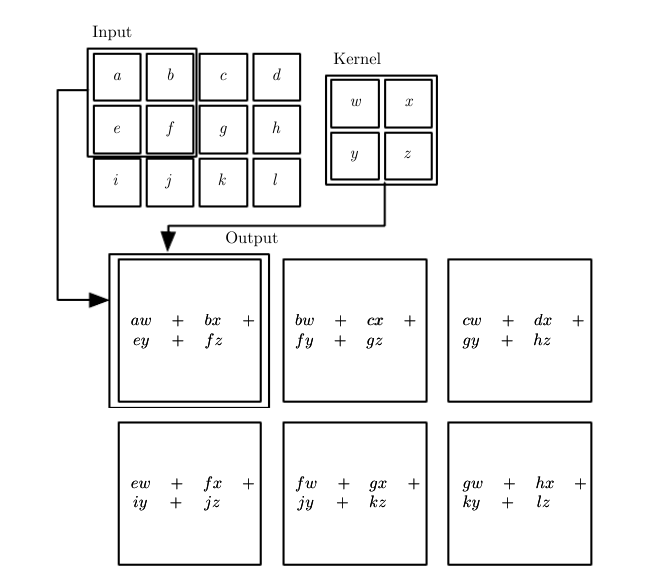
\includegraphics[width=0.6\textwidth]{src/assets/fundamentacao/convolution_operation.png}
    \captionsetup{justification=raggedright}
    \caption*{Fonte: \citefigure{DeeplearningLC}}
    \label{fig:convolution_operation}
\end{figure}

\noindent Em vez de conectar cada neurônio de uma camada a todos os neurônios da camada anterior, os neurônios em uma camada convolucional são conectados apenas a uma região local (conexões locais) \cite{DeeplearningLC}. A entrada líquida (\textit{net input}) em um neurônio convolucional é:

\begin{equation}
z_{x,y}^{\ell} = b^{\ell} + \sum_{l,k} w_{l,k}^{\ell} \cdot a_{x-l,y-k}^{\ell-1}
\end{equation}
\addEquacao{Entrada Líquida em Camada Convolucional}{5}

\noindent onde $z_{x,y}^{\ell}$ é a entrada na posição $(x,y)$ da camada $\ell$, $b^{\ell}$ é o viés (\textit{bias}), $w_{l,k}^{\ell}$ são os pesos do \textit{kernel} e $a_{x-l,y-k}^{\ell-1}$ são as ativações da camada anterior. Todas as unidades de um mesmo mapa de características compartilham o mesmo conjunto de pesos, o que reduz o número de parâmetros. Essa abordagem assume que um detector de características útil em uma parte da imagem será útil em outra parte. A camada de \textit{pooling} reduz a dimensão espacial dos mapas de características e torna a representação mais compacta e robusta a pequenas translações. Uma CNN típica consiste em estágios de camadas convolucionais seguidas por camadas de \textit{pooling}, e termina em camadas totalmente conectadas para a classificação.

Na convolução, cada elemento do mapa de características de saída depende apenas de uma região local da entrada e dos pesos do \textit{kernel} compartilhado, e não dos demais elementos da mesma camada. Essa independência de dados entre elementos de saída é o que permite calcular a camada em paralelo na GPU (\autoref{sec:paralelismo}).

A evolução das arquiteturas de CNNs é marcada pelo aumento progressivo da profundidade. Redes pioneiras como a LeNet-5 demonstraram a eficácia da combinação de camadas convolucionais e de \textit{pooling} no reconhecimento de caracteres \cite{Gradient-basedlearningappliedtodocumentrecognition}. A VGG mostrou que redes profundas podiam ser construídas com filtros pequenos ($3 \times 3$) \cite{VeryDeepConvolutionalNetworksforLarge-ScaleImageRecognition}. A GoogLeNet introduziu os módulos \textit{Inception}, que executam convoluções de diferentes tamanhos em paralelo \cite{szegedy2014goingdeeperconvolutions}.

\subsubsection{Aplicações de CNNs}

As CNNs são usadas em várias aplicações:

\begin{itemize}
    \item \textbf{Classificação de Imagens}: Atribui um único rótulo a uma imagem inteira \cite{NIPS2012_c399862d}.

    \item \textbf{Segmentação Semântica}: Classifica cada pixel de uma imagem em uma categoria específica \cite{Farabet6338939}. Em sensoriamento remoto, é usada no mapeamento de cobertura do solo \cite{rs16152729}.

    \item \textbf{Detecção de Objetos}: Localiza múltiplos objetos em uma imagem por meio de caixas delimitadoras (\textit{bounding boxes}) e classifica cada um \cite{sermanet2014overfeatintegratedrecognitionlocalization}.

    \item \textbf{Análise de Imagens Hiperespectrais}: Em imagens hiperespectrais, que contêm centenas de bandas espectrais, as CNNs extraem características espectrais e espaciais \cite{Li2019DeepLF}. A Figura \ref{fig:cnn1d_hsi} ilustra uma arquitetura CNN 1D para classificação de HSIs, do pré-processamento por PCA às camadas convolucionais 1D e densas que produzem a classificação.
\end{itemize}

\begin{figure}[H]
    \centering
    \captionsetup{justification=centering}
    \caption{Arquitetura CNN 1D para classificação de imagens hiperespectrais: pré-processamento PCA seguido de 4 camadas convolucionais 1D e camadas densas para classificação}
    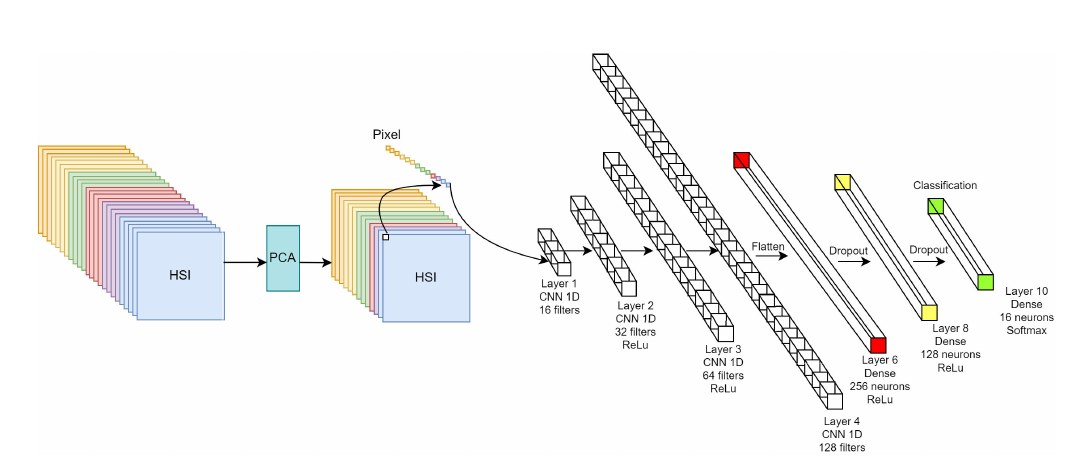
\includegraphics[width=0.95\textwidth]{src/assets/fundamentacao/cnn1d_hsi_architecture.png}
    \captionsetup{justification=raggedright}
    \caption*{Fonte: \citefigure{Viel10064297}}
    \label{fig:cnn1d_hsi}
\end{figure}

\section{Processamento Paralelo em GPUs}
\label{sec:paralelismo}

Neste trabalho, a CNN é treinada em GPU, exceto nas medições de paralelismo, feitas em CPU (\autoref{sec:resParalelismo}), e a segmentação é sempre executada em CPU. A arquitetura da GPU e o modelo de programação CUDA explicam por que as convoluções da rede se paralelizam bem, e a independência entre as etapas do fluxo define as demais estratégias de paralelização.

\subsection{Arquitetura de GPUs e CUDA Cores}

As Unidades de Processamento Gráfico (GPUs) evoluíram de aceleradores gráficos especializados para processadores paralelos de propósito geral \cite{CUDA_Programming}. Enquanto uma CPU tem tipicamente dezenas de núcleos otimizados para execução sequencial com baixa latência, uma GPU NVIDIA tem milhares de núcleos de processamento mais simples, os \textit{CUDA cores}, organizados em unidades chamadas \textit{Streaming Multiprocessors} (SMs) \cite{CUDA_Programming}.

Cada \textit{CUDA core} executa operações aritméticas de ponto flutuante, como soma, multiplicação e a operação fusionada de multiplicação e soma (FMA). Os \textit{CUDA cores} de um SM seguem o modelo SIMT (\textit{Single Instruction, Multiple Threads}): grupos de 32 threads, chamados \textit{warps}, executam a mesma instrução ao mesmo tempo sobre dados diferentes \cite{CUDA_Programming}. Essa arquitetura é eficiente para operações com paralelismo de dados, em que a mesma operação é aplicada a muitos elementos independentes.

A plataforma CUDA (\textit{Compute Unified Device Architecture}), desenvolvida pela NVIDIA, fornece um modelo de programação que permite explorar o paralelismo das GPUs em aplicações de computação geral \cite{CUDA_Programming}. O modelo de execução organiza as threads em três níveis: threads individuais são agrupadas em blocos, e os blocos, em grades. Como o hardware distribui os blocos entre os SMs disponíveis, o mesmo programa se adapta a GPUs com números diferentes de SMs \cite{CUDA_Architecture}.

\subsection{Paralelização de Operações de Convolução}

A operação de convolução em CNNs apresenta características intrínsecas que a tornam altamente paralelizável \cite{cuConv}. Para uma camada convolucional com entrada $X$ de dimensões $(N, C_{in}, H, W)$ (lote, canais de entrada, altura, largura), filtros $K$ de dimensões $(C_{out}, C_{in}, k_h, k_w)$ e saída $Y$ de dimensões $(N, C_{out}, H_{out}, W_{out})$, cada elemento de saída é calculado como:

\begin{equation}
Y[n, c_{out}, i, j] = \sum_{c_{in}=0}^{C_{in}-1} \sum_{m=0}^{k_h-1} \sum_{l=0}^{k_w-1} X[n, c_{in}, i+m, j+l] \cdot K[c_{out}, c_{in}, m, l] + b[c_{out}]
\end{equation}

Nenhum elemento $Y[n, c_{out}, i, j]$ depende do cálculo de outro elemento da saída; os $N \times C_{out} \times H_{out} \times W_{out}$ elementos podem, portanto, ser calculados simultaneamente, se houver recursos computacionais suficientes. Na CNN 1D, a dimensão da altura desaparece e a propriedade se mantém: cada posição do mapa de características ao longo do espectro pode ser calculada em paralelo.

Na prática, \textit{frameworks} de aprendizado profundo como TensorFlow e PyTorch usam a biblioteca cuDNN da NVIDIA, que escolhe, para cada configuração da camada, um entre vários algoritmos de convolução \cite{Jorda_cuDNN}.

\subsection{Estratégias de Paralelização para o Fluxo de Classificação}

O treinamento e a inferência de CNNs admitem paralelismo em mais de um nível \cite{Aach2025, Nandan10910577}. Os três a seguir são os relevantes para o fluxo de classificação de HSIs.

\textbf{Paralelismo de Dados}: Réplicas do modelo processam subconjuntos diferentes dos dados ao mesmo tempo, e os gradientes são agregados para atualizar os pesos. A MirroredStrategy do TensorFlow e a DataParallel do PyTorch implementam essa estratégia, mais útil quando o conjunto de dados é grande e há várias GPUs disponíveis \cite{Nandan10910577}. A partição da cena, uma das estratégias deste trabalho, também divide os dados entre unidades de execução, mas sem agregar gradientes: cada parte da cena é processada por uma thread ou por um processo (\autoref{sec:desParalelismo}).

\textbf{Paralelismo Intra-Camada}: Dentro de uma camada convolucional, os elementos de saída são calculados em paralelo nos \textit{CUDA cores}. As implementações em GPU, como a cuDNN, exploram esse paralelismo automaticamente, sem intervenção do programador.

\textbf{Paralelismo entre Etapas}: Etapas que não dependem uma da outra podem ser executadas concorrentemente. No fluxo de \citeonline{Souza2023}, isso ocorre em dois pontos. Na preparação dos dados, o ramo espectral, que reduz o espectro por PCA, e o ramo espacial, que compõe as três primeiras componentes principais e segmenta a imagem, partem da mesma cena e só se reúnem na montagem das entradas da rede. Na inferência, a segmentação, executada em CPU pelo OpenCV, e as convoluções da rede também são independentes: as convoluções não usam o mapa de segmentação, e a sincronização só é necessária na concatenação, que precisa do identificador do superpixel de cada pixel. Essas duas oportunidades correspondem, neste trabalho, ao paralelismo entre os ramos do pré-processamento e à fusão concorrente (\autoref{sec:desParalelismo}); a biblioteca padrão do Python oferece threads e processos para executá-las \cite{Python_Threading}.

\section{Concorrência em CPU}
\label{sec:concorrencia}

O paralelismo entre etapas exige os conceitos clássicos de concorrência dos sistemas operacionais. Na fusão espectral-espacial, a segmentação, executada em CPU pelo OpenCV, e as convoluções da rede só se encontram no ponto de fusão.

\subsection{Threads, Processos e o GIL}

Um processo é um programa em execução com espaço de endereçamento próprio; uma thread é um fluxo de execução dentro de um processo, e as threads de um mesmo processo compartilham sua memória \cite{Silberschatz2018}. Criar uma thread é barato e não copia dados; processos são isolados, e trocar dados entre eles exige serializá-los e copiá-los, com custo proporcional ao volume transferido.

No CPython, o interpretador de referência do Python, o \textit{Global Interpreter Lock} (GIL) garante que apenas uma thread execute \textit{bytecode} Python por vez \cite{PEP703}. Código Python puro em várias threads, portanto, não executa em paralelo, enquanto código nativo que libera o GIL durante o cálculo, como as rotinas do NumPy, o OpenCV e os \textit{kernels} do PyTorch, executa (\autoref{fig:gil}). O ganho das threads depende da fração do trabalho que acontece fora do interpretador.

\begin{figure}[H]
    \centering
    \captionsetup{justification=centering}
    \caption{Quatro threads de um processo executando código Python e código nativo que libera o GIL}
    \begin{tikzpicture}[font=\footnotesize, x=0.8cm, y=0.5cm]
        \foreach \dx/\titulo in {0/{Código Python: o GIL alterna as threads}, 9/{Código nativo: o GIL é liberado}} {
            \node[anchor=south west, font=\footnotesize\bfseries] at (\dx-0.6, 3.7) {\titulo};
            \foreach \i in {1,...,4} {
                \node[anchor=east] at (\dx-0.1, 4-\i) {T\i};
                \draw[black!20] (\dx, 4-\i) -- (\dx+8, 4-\i);
            }
            \draw[-{Stealth[length=2mm]}] (\dx, -0.9) -- (\dx+8, -0.9) node[below left] {tempo};
        }
        \foreach \k in {0,...,15} {
            \pgfmathtruncatemacro{\linha}{mod(\k,4)+1}
            \fill[azulfig] ({0.5*\k}, {4-\linha-0.3}) rectangle ++(0.45, 0.6);
        }
        \foreach \i in {1,...,4} {
            \fill[laranjafig] (9, {4-\i-0.3}) rectangle ++(2.0, 0.6);
        }
    \end{tikzpicture}
    \captionsetup{justification=raggedright}
    \caption*{Fonte: Elaborada pelo autor}
    \label{fig:gil}
\end{figure}

\subsection{Exclusão Mútua e Variáveis de Condição}

Quando duas threads acessam o mesmo dado e ao menos uma o modifica, o resultado pode depender da ordem de execução, situação chamada de condição de corrida. O trecho que acessa o dado compartilhado é a seção crítica, protegida em geral por um mutex (de \textit{mutual exclusion}): uma trava que só uma thread detém por vez \cite{Silberschatz2018}. O mutex garante exclusão, mas não ordem: se a thread consumidora adquirir a trava antes da produtora, lerá o dado ainda não produzido. Para impor ordem, usa-se uma variável de condição, associada ao mutex e a um predicado: a consumidora verifica o predicado e, se ele for falso, espera com a trava liberada, até que a produtora atualize o dado e a notifique. Esse conjunto corresponde ao conceito de monitor \cite{Hoare1974Monitors}. A barreira, outra primitiva usada neste trabalho, bloqueia um grupo de threads até que todas cheguem ao mesmo ponto.

\subsection{Lei de Amdahl e \textit{Speedup}}

O \textit{speedup} é a razão entre o tempo de uma versão de referência e o da versão paralela, e a escolha da referência é parte da medição: comparar uma versão paralela em CPU com uma sequencial em GPU mede também a diferença de dispositivo. Pela lei de Amdahl \cite{Amdahl1967}, se uma fração $p$ do tempo de execução pode ser dividida entre $N$ unidades, o \textit{speedup} máximo é:

\begin{equation}
S(N) = \frac{1}{(1 - p) + \dfrac{p}{N}}
\end{equation}
\addEquacao{Lei de Amdahl}{13}

\noindent Dois corolários orientam este trabalho. Paralelizar uma etapa que responde por 1\% do tempo total muda esse tempo em no máximo 1\%. E, quando duas etapas independentes de durações $T_1$ e $T_2$ passam a ser executadas concorrentemente, o \textit{speedup} não pode exceder:

\begin{equation}
S_{\max} = \frac{T_1 + T_2}{\max(T_1, T_2)}
\end{equation}
\addEquacao{Teto do Paralelismo entre Duas Etapas}{14}

\noindent que vale 2 apenas quando as etapas têm a mesma duração. A distância até esse teto vem da sobrecarga (\textit{overhead}) de coordenar a execução, isto é, criar threads ou processos, serializar dados e sincronizar, e da contenção: tarefas que disputam a banda de memória, o \textit{cache} ou o GIL ficam mais lentas do que seriam sozinhas.

\section{Otimização de Hiperparâmetros}
\label{sec:fundHPO}

Hiperparâmetros são as escolhas feitas antes do treino, como a taxa de aprendizado, o \textit{dropout}, o tamanho do lote, o número de componentes do PCA e os parâmetros do segmentador; os parâmetros, os pesos, são o que o treino aprende. A Otimização de Hiperparâmetros (HPO) automatiza a escolha: cada avaliação de uma combinação, chamada \textit{trial}, consiste em treinar e validar um modelo \cite{WU201926}.

A busca em grade avalia todas as combinações de um espaço discreto e fica inviável rapidamente, porque o número de combinações é o produto do número de valores de cada hiperparâmetro. A busca aleatória sorteia combinações e, com o mesmo orçamento, encontra configurações tão boas quanto as da grade ou melhores, porque poucos hiperparâmetros costumam importar e o sorteio testa mais valores distintos de cada um \cite{Bergstra2012Random}. A Otimização Bayesiana usa os \textit{trials} já observados para decidir o próximo. Na forma clássica, ela modela a função objetivo por um processo gaussiano e escolhe o próximo \textit{trial} por uma função de aquisição, que equilibra exploração e explotação \cite{WU201926}; o \textit{Tree-structured Parzen Estimator} (TPE) estima as densidades $l(x)$ e $g(x)$ dos hiperparâmetros entre os melhores \textit{trials} e entre os demais e propõe a combinação que maximiza $l(x)/g(x)$ \cite{Bergstra2011TPE}, e a biblioteca Optuna o implementa \cite{Akiba2019Optuna}. Os algoritmos genéticos mantêm uma população de candidatos e a aprimoram a cada geração por seleção, cruzamento e mutação; o elitismo preserva os melhores de uma geração para a seguinte \cite{Holland1975}.

A seleção deve usar exclusivamente o conjunto de validação, porque escolher pelo teste o transforma em parte do ajuste. Como cada \textit{trial} é um treino, o custo pode ser reduzido avaliando os candidatos com poucas épocas e retreinando só o vencedor, como fazem os agendadores ASHA e RASDA (\autoref{sec:trabRel}) \cite{Aach2025}. O risco é que a ordenação obtida com poucas épocas não se mantenha com o treino completo, o que foi medido neste trabalho com 10, 40 e 200 épocas por \textit{trial} (\autoref{tab:estrategias}).

\section{Trabalhos Relacionados}
\label{sec:trabRel}

Os trabalhos relacionados foram escolhidos por tratarem de otimização: da busca de hiperparâmetros, do paralelismo no treinamento de CNNs e do próprio fluxo de classificação de HSIs que este trabalho toma como ponto de partida.

\subsection{Protocolo de Análise}

A busca foi feita no Portal de Periódicos da CAPES, com acesso fornecido pela UNIVALI, abrangendo bases como IEEE, Science Direct e ACM, e no Google Scholar, que levou a resultados de outras fontes, como Springer e Taylor \& Francis. Não se trata de uma revisão sistemática: a seleção foi intencional, guiada pelos critérios a seguir.

A seleção dos trabalhos foi baseada em:
(\textit{i}) implementação de uma arquitetura de classificação de HSI;
(\textit{ii}) apresentação detalhada da arquitetura;
(\textit{iii}) implementação de um algoritmo para processamento espectral e espacial; e
(\textit{iv}) apresentação das métricas empregadas para avaliar precisão e/ou tempo de processamento.
Na triagem, foram descartadas as arquiteturas que empregam mais de um modelo de ML, como uma rede convolucional encadeada a uma rede recorrente, ou um conjunto grande de algoritmos de processamento. O interesse deste trabalho está no algoritmo espacial (a segmentação) acoplado a uma rede simples, e não na combinação de muitos algoritmos para chegar ao estado da arte.

Foram selecionados três trabalhos. Apenas o de \citeonline{Souza2023} atende aos quatro critérios. Os de \citeonline{Aach2025} e \citeonline{Nandan10910577} não tratam de HSIs nem de processamento espectral-espacial (critérios \textit{i} e \textit{iii}) e foram incluídos pelos temas de otimização que este trabalho aplica ao fluxo de \citeonline{Souza2023}: a otimização de hiperparâmetros em escala, no primeiro, e o paralelismo no treinamento de CNNs, no segundo (\autoref{tab:trabRel}).

\subsection{Parallel and Scalable Hyperparameter Optimization for Distributed Deep Learning Methods on High-Performance Computing Systems}

\citeonline{Aach2025} propõe métodos para realizar Otimização de Hiperparâmetros (HPO) de forma eficiente em sistemas de Computação de Alto Desempenho (HPC) com grandes volumes de dados científicos, que vão de centenas de gigabytes a vários terabytes. O desempenho de redes neurais depende dos hiperparâmetros, que incluem parâmetros arquiteturais (número de camadas, funções de ativação, tamanho de \textit{kernels}) e parâmetros do otimizador (taxa de aprendizado, \textit{weight decay}, \textit{momentum}, tamanho do lote).

O estudo investiga espaços de busca multidimensionais em três domínios. Para Visão Computacional usando ResNet50 no ImageNet, os hiperparâmetros otimizados incluem: taxa de aprendizado (log[$10^{-5}$, $1$]), \textit{weight decay} (log[$0$, $10^{-1}$]), épocas de \textit{warm-up} inicial ([$1$-$5$]), tipo de otimizador (SGD, Adam), inicialização de camadas (Kaiming, Xavier), função de ativação (ReLU, LeakyReLU, SELU, Tanh, Sigmoid) e tamanho do \textit{kernel} de convolução ([$5$, $7$, $9$]). No domínio de Fluidodinâmica Computacional (CFD), com 8,3 TB de dados e um autoencoder convolucional, inclui-se, além dos hiperparâmetros anteriores, o \textit{re-scaling warm-up} ([$1$, $2$]), que ajusta gradualmente a taxa de aprendizado à medida que o número de GPUs aumenta. Para Manufatura Aditiva (AM), com SwinTransformer, o espaço adiciona: tamanho do \textit{patch} ([$2$, $4$]), profundidade ([$1$, $2$, $4$]), número de cabeças de atenção ([$3$, $6$, $12$, $24$]) e \textit{MLP ratio} ([$1.0$, $2.0$, $3.0$, $4.0$]).

O autor desenvolve o RASDA (\textit{Resource-Adaptive Successive Doubling Algorithm}), um agendador escalável que realoca GPUs durante a otimização, tirando recursos dos \textit{trials} de baixo desempenho para acelerar os mais promissores. Na validação experimental, em até 1024 GPUs, o RASDA foi até $1,9\times$ mais rápido que o ASHA padrão e, no experimento CFD, chegou a um erro quadrático médio de $3,63 \times 10^{-7}$.

A Figura~\ref{fig:rasda_comparison} mostra o que distingue o RASDA: enquanto o ASHA mantém constantes o lote global e a alocação de GPUs, o RASDA aumenta progressivamente os dois à medida que identifica \textit{trials} promissores. No caso CFD, o lote global cresce de 16 para 128, e as GPUs por \textit{trial}, de 8 para 64.

\begin{figure}[htb]
\centering
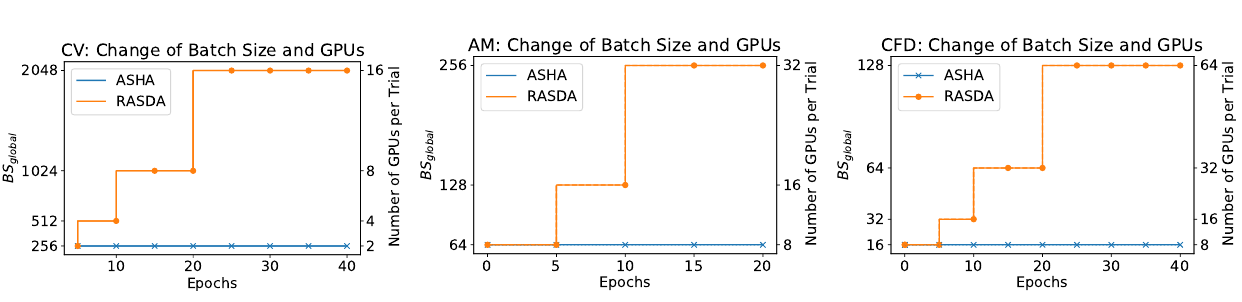
\includegraphics[width=\textwidth]{src/assets/trabalhos_relacionados/rasda_comparison.png}
\caption{Comparação entre o tamanho global do lote e o número de GPUs por \textit{trial} no ASHA e no RASDA, nos diferentes casos de aplicação}
\caption*{Fonte: \citefigure{Aach2025}}
\label{fig:rasda_comparison}
\end{figure}

\subsection{Comparative Analysis of TensorFlow and PyTorch for Image Classification using CNN with Parallelism Strategies}

\citeonline{Nandan10910577} investigou como o paralelismo de dados afeta o tempo de treinamento e a acurácia de CNNs de classificação de imagens em dois \textit{frameworks}, comparando a MirroredStrategy do TensorFlow com a DataParallel do PyTorch nos conjuntos CIFAR-10 e CIFAR-100. O modelo tem três camadas convolucionais seguidas por duas camadas densas. Cada \textit{framework} foi testado em modo sequencial e com paralelismo de dados, e foram coletados a acurácia de teste, o tempo de treinamento e as curvas de aprendizado.

No CIFAR-10, o paralelismo aumentou o tempo de treinamento, o que o autor atribui à sobrecarga de comunicação: o TensorFlow passou de 84,53 s para 144,6 s, e o PyTorch, de 210,42 s para 253,2 s. Com paralelismo, o PyTorch obteve acurácia maior (0,717, contra 0,680 do TensorFlow). As curvas das Figuras \ref{fig:tensorflow_results} e \ref{fig:pytorch_results} mostram, nos dois \textit{frameworks}, a acurácia de treino subindo ao longo das dez épocas enquanto a de validação se estabiliza perto de 0,70, com distância crescente entre as duas; as curvas do PyTorch com e sem paralelismo são quase iguais, e as do TensorFlow diferem mais entre si. No CIFAR-100, o paralelismo reduziu os tempos de treinamento: o do TensorFlow de 224,23 s para 202,84 s, e o do PyTorch de 373,45 s para 341,4 s. A acurácia do PyTorch subiu de 0,43 para 0,45, e a do TensorFlow caiu de 0,46 para 0,42.

O autor associa o TensorFlow à prototipagem rápida e o PyTorch a aplicações em que a acurácia é prioritária, mas os experimentos medem apenas tempo de treinamento e acurácia no CIFAR; nada neles avalia prototipagem ou uso em produção. Do mesmo modo, o paralelismo aumentou o tempo no CIFAR-10 e o reduziu no CIFAR-100, mas os dois conjuntos têm o mesmo número e o mesmo tamanho de imagens e diferem apenas no número de classes, de modo que esses resultados não bastam para atribuir a diferença à escala do problema. O que eles mostram, e que interessa a este trabalho, é que a sobrecarga de coordenar a execução paralela pode superar o ganho.

\begin{figure}[H]
    \centering
    \captionsetup{justification=centering}
    \caption{Curvas de acurácia de treino e de validação do TensorFlow com as estratégias sequencial e de paralelismo de dados no CIFAR-10}
    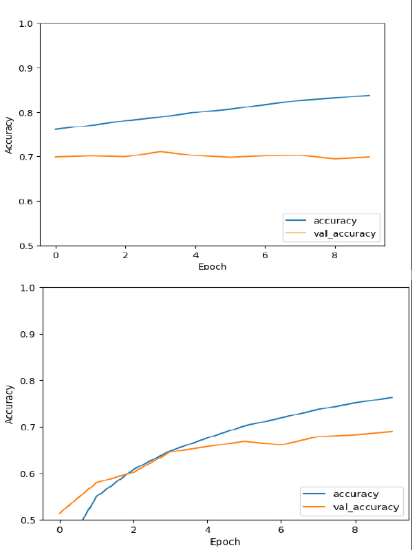
\includegraphics[width=0.33\textwidth]{src/assets/trabalhos_relacionados/comparative_analysis_of_tensorflow_and_pytorch_for_image_classification_using_cnn_with_parallelism_strategies_1.png}\\
    \captionsetup{justification=raggedright}
    \caption*{Fonte: \citefigure{Nandan10910577}}
    \label{fig:tensorflow_results}
\end{figure}

\begin{figure}[H]
    \centering
    \captionsetup{justification=centering}
    \caption{Curvas de acurácia de treino e de validação do PyTorch com as estratégias sequencial e de paralelismo de dados no CIFAR-10}
    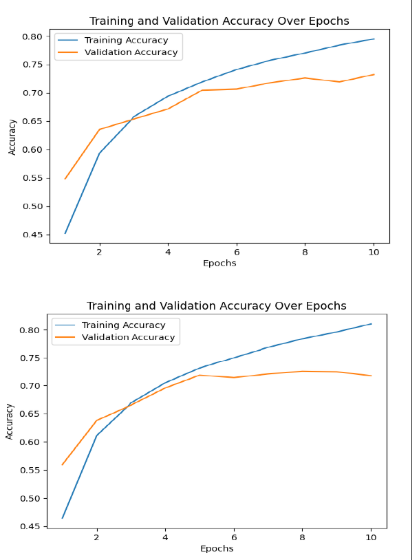
\includegraphics[width=0.33\textwidth]{src/assets/trabalhos_relacionados/comparative_analysis_of_tensorflow_and_pytorch_for_image_classification_using_cnn_with_parallelism_strategies_2.png}\\
    \captionsetup{justification=raggedright}
    \caption*{Fonte: \citefigure{Nandan10910577}}
    \label{fig:pytorch_results}
\end{figure}

\subsection{Avaliação de Fusão de Dados Espaciais com Espectrais para Classificação de Imagens Hiperespectrais}

O trabalho de \citeonline{Souza2023} é o ponto de partida deste estudo. O autor aborda a classificação de HSIs, em que há um compromisso entre complexidade computacional e acurácia, e observa que os métodos tradicionais se concentram nas características espectrais e subutilizam o contexto espacial, que pode melhorar a distinção entre classes. Os objetivos são avaliar o impacto do pré-processamento espacial na classificação por aprendizado de máquina, integrar a segmentação SEEDS a uma CNN 1D por concatenação, comparar o resultado com modelos de base e com o estado da arte, e quantificar o custo computacional da abordagem.

A metodologia propõe uma arquitetura híbrida que combina uma CNN 1D, para a classificação espectral, com o SEEDS, para a segmentação espacial. A Figura \ref{fig:metodologia_souza} mostra o fluxo completo, da separação dos conjuntos de dados à extração das métricas de avaliação. O processamento tem dois ramos independentes, executados em sequência: o ramo superior realiza PCA, definição de parâmetros, segmentação e concatenação das características espaciais; o ramo inferior executa PCA e vetorização, divisão dos dados de treino e classificação pela CNN 1D. Na implementação original, a CNN 1D tem quatro camadas convolucionais, com 16, 32, 64 e 64 filtros, seguidas por duas camadas densas, de 128 e 64 neurônios, e pela camada de saída (\autoref{tab:camadas}). A fusão é feita por uma camada de concatenação, que junta às características extraídas pelas convoluções o identificador do superpixel do pixel. Os hiperparâmetros da rede e do SEEDS foram ajustados manualmente: o autor relata ter alterado, por conjunto de dados, a paciência da parada antecipada e outros parâmetros de treino ao buscar o melhor resultado \cite{Souza2023}.

\begin{figure}[H]
    \centering
    \captionsetup{justification=centering}
    \caption{Fluxograma da metodologia proposta, com os ramos espacial e espectral, a fusão via concatenação, a classificação e a validação iterativa do modelo}
    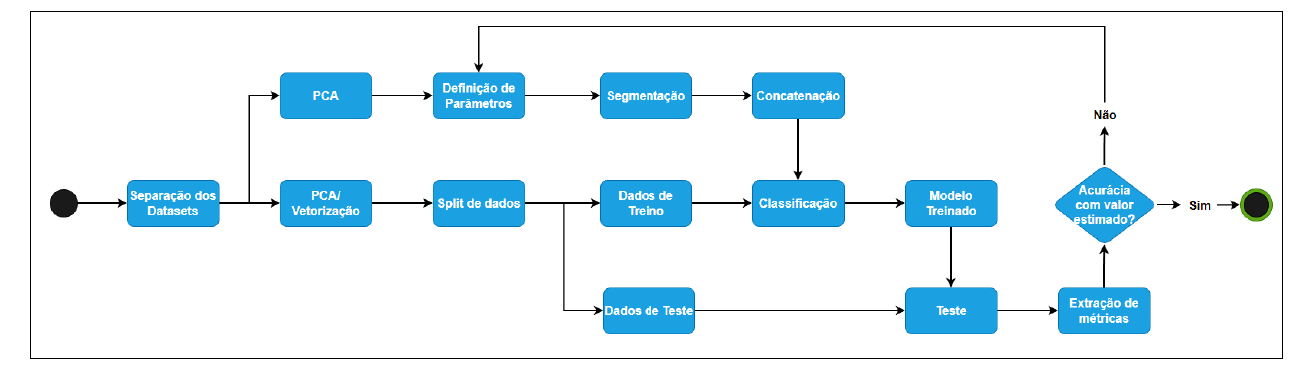
\includegraphics[width=\textwidth]{src/assets/trabalhos_relacionados/metodologia_souza.png}
    \captionsetup{justification=raggedright}
    \caption*{Fonte: \citefigure{Souza2023}}
    \label{fig:metodologia_souza}
\end{figure}

A validação experimental foi conduzida em três cenas: Indian Pines (21.025 pixels, 10.249 rotulados, 16 classes), Salinas Valley (111.104 pixels, 54.129 rotulados, 16 classes) e University of Pavia (207.400 pixels, 42.776 rotulados, 9 classes). As métricas avaliadas incluem Acurácia Geral (OA), Acurácia Média (AA), coeficiente Kappa, tempo de inferência e uso de memória. Com a fusão SEEDS, o autor reporta OA de 0,9142, AA de 0,8956 e Kappa de 0,9019 em Indian Pines, OA de 0,9928 em University of Pavia e OA de 0,9965 em Salinas Valley (\autoref{tab:linhaBase}); em Indian Pines, a fusão acrescentou 8,33, 8,79 e 9,47 pontos percentuais de OA, AA e Kappa à mesma rede sem a informação espacial. Essa configuração, com a fusão, é a referência contra a qual os ganhos deste trabalho são medidos. O fluxograma da Figura \ref{fig:metodologia_souza} mostra ainda o processo iterativo de treinamento, teste e extração de métricas, com validação baseada em um valor estimado de acurácia.

\subsection{Análise Comparativa dos Trabalhos Relacionados}

O \autoref{tab:trabRel} compara os três trabalhos com este. Os de \citeonline{Aach2025} e \citeonline{Nandan10910577} tratam de otimização, de hiperparâmetros em escala e de paralelismo no treinamento, respectivamente, mas em problemas de visão computacional, fluidodinâmica e manufatura aditiva, sem HSIs nem segmentação. O de \citeonline{Souza2023} trata de HSIs com fusão espectral-espacial, mas executa as etapas em sequência, ajusta os hiperparâmetros à mão e usa um único segmentador. Nenhum dos três combina, no mesmo fluxo de classificação de HSIs, a busca automática de hiperparâmetros da rede e do segmentador, a comparação de segmentadores sob a mesma otimização e o paralelismo entre as etapas; é essa a lacuna que este trabalho ocupa.

\begin{quadro}[H]
    \centering
    \caption{Comparação dos trabalhos relacionados}
    \resizebox{\textwidth}{!}{%
    \begin{tabular}{|p{0.20\textwidth}|p{0.19\textwidth}|p{0.19\textwidth}|p{0.19\textwidth}|p{0.19\textwidth}|}
        \hline
        \rowcolor[HTML]{EFEFEF}
        \textbf{Característica} & \textbf{\cite{Aach2025}} & \textbf{\cite{Nandan10910577}} & \textbf{\cite{Souza2023}} & \textbf{Este Trabalho} \\
        \hline
        \textbf{Arquitetura de IA} & 
        ResNet50 (ImageNet), autoencoder convolucional (CFD) e SwinTransformer (AM) &
        CNN customizada&
        CNN 1D& 
        CNN 1D otimizada com fusão espectral-espacial \\
        \hline
        \textbf{Processamento Paralelo} & 
        Sim. RASDA&
        Sim. Paralelismo de dados (MirroredStrategy e DataParallel) &
        Não. Ramos independentes, executados em sequência &
        Sim. Threads e processos: entre os ramos do pré-processamento, por partição da cena e na fusão concorrente\\
        \hline
        \textbf{Segmentação} & 
        Não aplicado & 
        Não aplicado & 
        Sim. SEEDS ajustado manualmente & 
        Sim. SEEDS, SLIC, LSC e Watershed sob otimização conjunta \\
        \hline
        \textbf{HPO} & 
        Sim. ASHA e RASDA &
        Não abordada &
        Não. Ajuste manual por conjunto de dados &
        Sim. Busca aleatória, TPE e algoritmo genético para CNN e segmentação \\
        \hline
        \textbf{Métricas} & 
        Val MSE, Test MSE, Runtime, Relative Error & 
        Test Accuracy, Training Time, Val Accuracy & 
        OA, AA, Kappa, Tempo, Memória & 
        OA, AA, Kappa, Tempo, Memória, \textit{Speedup} \\
        \hline
        \textbf{Datasets} & 
        ImageNet, CFD, RAISE-LPBF& 
        CIFAR-10, CIFAR-100& 
        Indian Pines, Salinas, Pavia& 
        Indian Pines, Salinas Valley, University of Pavia \\
        \hline
        \textbf{Tecnologias} & 
        Python, PyTorch, Horovod, DeepSpeed, Ray Tune, CUDA 11.5, NVIDIA DALI& 
        Python, TensorFlow, PyTorch, Keras, CUDA& 
        Python, TensorFlow, Keras, scikit-learn, OpenCV, Google Colab&
        Python, PyTorch, scikit-learn, OpenCV, Optuna\\
        \hline
    \end{tabular}%
    }
    \captionsetup{justification=raggedright}
    \caption*{Fonte: Elaborado pelo autor}
    \label{tab:trabRel}
\end{quadro}